% ============================================================
%  LoRA Continual Learning for BlueROV2 AUV Control
%  Full paper — IEEE Transactions / ICRA style
% ============================================================

\documentclass[journal]{IEEEtran}

% ── Packages ─────────────────────────────────────────────────────────────────
\usepackage[T1]{fontenc}
\usepackage[utf8]{inputenc}
\usepackage{amsmath, amssymb, mathtools}
\usepackage{bm}              % bold math
\usepackage{graphicx}
\usepackage{subcaption}
\usepackage{booktabs}        % toprule / midrule / bottomrule
\usepackage{multirow}
\usepackage{xcolor}
\usepackage{hyperref}
\usepackage{algorithm}
\usepackage{algpseudocode}
\usepackage{siunitx}         % SI units
\usepackage{cite}
\usepackage{url}
\usepackage{float}

% ── Macros ───────────────────────────────────────────────────────────────────
\newcommand{\R}{\mathbb{R}}
\newcommand{\norm}[1]{\left\lVert #1 \right\rVert}
\newcommand{\abs}[1]{\left| #1 \right|}
\newcommand{\bx}{\bm{x}}
\newcommand{\bu}{\bm{u}}
\newcommand{\bnu}{\bm{\nu}}
\newcommand{\boldeta}{\bm{\eta}}
\newcommand{\blora}[1]{\Delta\bm{W}_{#1}}

% ── Metadata ─────────────────────────────────────────────────────────────────
\title{Continual Learning with Low-Rank Adaptation for\\
       Autonomous Underwater Vehicle Control:\\
       Disturbance Compensation via Online Inverse-Model Adaptation}

\author{%
  \IEEEauthorblockN{Abdelhakim~Amer}\\
  \IEEEauthorblockA{Department of Engineering Cybernetics\\
    Norwegian University of Science and Technology (NTNU)\\
    Trondheim, Norway\\
    \textit{abdelhakim.amer@ntnu.no}}
}

\markboth{IEEE Transactions on Control Systems Technology}{%
  A.\ Amer: LoRA-CL for BlueROV2}

% ─────────────────────────────────────────────────────────────────────────────
\begin{document}
\maketitle

% ─────────────────────────────────────────────────────────────────────────────
\begin{abstract}
Autonomous Underwater Vehicles (AUVs) operate in environments characterised
by time-varying hydrodynamic disturbances, measurement noise, and model
uncertainty, making accurate trajectory tracking a persistent challenge.
Classical model-based controllers such as PID or inverse-dynamics controllers
rely on accurate plant models that may degrade under ocean currents or payload
changes. Deep-learning controllers pre-trained on clean data suffer
catastrophic forgetting when deployed under distribution shift.
We propose \emph{LoRA-CL}, a continual-learning framework that combines a
pre-trained neural inverse model with Low-Rank Adaptation (LoRA) adapters,
enabling lightweight online adaptation without overwriting previously
acquired knowledge. Three continual-learning strategies are evaluated:
LoRA with Experience Replay (LoRA-ER), Elastic Weight Consolidation
(LoRA-EWC), and Averaged Gradient Episodic Memory (LoRA-AGEM).
Experiments on the BlueROV2 Heavy simulation model along a Bernoulli
lemniscate trajectory demonstrate that LoRA-ER achieves the best overall
position tracking accuracy, reducing RMSE by up to \SI{95}{\percent}
relative to a frozen DNN baseline when ocean-current and parameter
uncertainty are introduced simultaneously. All three LoRA-CL variants
significantly outperform the DNN baseline while retaining performance in
disturbance-free phases, demonstrating forward transfer and the absence of
catastrophic forgetting. The entire framework is open-sourced at
\url{https://github.com/abdelhakim96/ContinualLearning_Drone}.
\end{abstract}

\begin{IEEEkeywords}
Autonomous underwater vehicles, continual learning, LoRA, inverse model
control, trajectory tracking, ocean current compensation, disturbance rejection.
\end{IEEEkeywords}

% ─────────────────────────────────────────────────────────────────────────────
\section{Introduction}
\label{sec:intro}
% ─────────────────────────────────────────────────────────────────────────────

Autonomous Underwater Vehicles (AUVs) are increasingly deployed for
inspection, survey, and intervention tasks in challenging marine environments.
Precise trajectory tracking is essential but difficult: ocean currents impose
time-varying body forces, biofouling gradually alters hydrodynamic
coefficients, and sensor noise degrades state estimates.

Classical control approaches—Proportional-Integral-Derivative (PID)
controllers and model-based inverse-dynamics controllers—offer predictable
behaviour but require accurate plant models that must be re-identified when
conditions change. Adaptive control and sliding-mode methods can handle
bounded uncertainty but often require explicit disturbance observers and
careful gain scheduling.

Data-driven approaches have demonstrated superior disturbance rejection by
learning residual dynamics directly from experience. However, standard neural
networks trained offline exhibit \emph{catastrophic forgetting}: when
fine-tuned on new conditions they overwrite previously learned knowledge,
leading to poor performance if the environment reverts to earlier conditions
\cite{mccloskey1989catastrophic}. This is particularly problematic for AUVs
that may transition between sheltered harbours, coastal currents, and deep
water over a single mission.

\emph{Continual learning} (CL) studies the problem of sequentially learning
from non-stationary data streams without forgetting. Successful CL
algorithms include Experience Replay (ER) \cite{rolnick2019experience},
Elastic Weight Consolidation (EWC) \cite{kirkpatrick2017overcoming}, and
Averaged Gradient Episodic Memory (A-GEM) \cite{chaudhry2019efficient}.

\emph{Low-Rank Adaptation} (LoRA) \cite{hu2022lora}, originally proposed for
efficient fine-tuning of large language models, provides an elegant foundation
for continual learning: by keeping the base model frozen and training only
small low-rank adapter matrices, LoRA naturally limits forgetting while
enabling rapid adaptation. The adapter parameter count is typically
$< 1\%$ of the full model, making online gradient steps computationally
tractable on embedded processors.

This paper makes the following contributions:
\begin{enumerate}
  \item We introduce \textbf{LoRA-CL} for AUV control: a continual-learning
        framework that wraps a pre-trained inverse-model MLP with LoRA
        adapters, enabling parameter-efficient online adaptation.
  \item We evaluate three CL strategies—LoRA-ER, LoRA-EWC, and LoRA-AGEM—in
        a systematic seven-phase benchmark covering noise, ocean current, and
        hydrodynamic uncertainty.
  \item We provide a comprehensive open-source implementation for the
        BlueROV2~Heavy platform, including the 4-DOF simulation model,
        trajectory generators, and all baseline controllers.
  \item We demonstrate that LoRA-CL achieves backward transfer (no forgetting
        in clean phases) and forward transfer (immediate improvement when
        disturbances recur) that static controllers and standard CL cannot match.
\end{enumerate}

% ─────────────────────────────────────────────────────────────────────────────
\section{Related Work}
\label{sec:related}
% ─────────────────────────────────────────────────────────────────────────────

\subsection{AUV Control}

PID control remains the industry standard for AUV path following
\cite{fossen2011handbook}. Adaptive PID and model-reference adaptive
controllers (MRAC) improve robustness at the cost of stability analysis
complexity \cite{fossen1999guidance}. Sliding-mode and backstepping
controllers have been applied to BlueROV2-class vehicles
\cite{cai2021adaptive}.

Neural network-based AUV controllers have attracted significant attention.
\citet{fan2018towards} used echo-state networks for disturbance compensation;
\citet{makavita2019experimental} combined a DNN with a model predictive
controller; \citet{carlucho2018incremental} applied reinforcement learning
for AUV velocity control. However, none address the non-stationary deployment
scenario considered here.

\subsection{Continual Learning}

Continual learning surveys \cite{parisi2019continual, delange2021continual}
classify approaches as: (a) replay-based (ER, generative replay); (b)
regularisation-based (EWC, SI, LwF); and (c) architecture-based
(progressive networks, PackNet). CL has been applied to robotics locomotion
\cite{kaplanis2019continual} and manipulation \cite{lesort2020continual}
but rarely to marine vehicles.

\subsection{Low-Rank Adaptation}

\citet{hu2022lora} showed that large language models can be fine-tuned
effectively with $r=4$ to $r=16$ LoRA rank, updating less than $0.1\%$
of parameters. LoRA has since been applied to vision transformers
\cite{zhu2023minigpt} and reinforcement learning
\cite{liang2024loradaptor}, but not, to our knowledge, to AUV control.

% ─────────────────────────────────────────────────────────────────────────────
\section{Problem Formulation}
\label{sec:problem}
% ─────────────────────────────────────────────────────────────────────────────

\subsection{BlueROV2 4-DOF Model}

We consider a simplified 4-DOF representation of the BlueROV2 Heavy AUV
that neglects roll and pitch (assumed stable due to meta-centric restoring
moments). The state vector is

\begin{equation}
  \bx = \bigl[\underbrace{x,\, y,\, z,\, \cos\psi,\, \sin\psi}_{\boldeta},\;
               \underbrace{u,\, v,\, w,\, r}_{\bnu}\bigr]^{\top} \in \R^9,
  \label{eq:state}
\end{equation}

where $\boldeta = (x,y,z,\psi)$ are the NED position and heading, encoded
with $(\cos\psi, \sin\psi)$ to avoid angle wrapping discontinuities, and
$\bnu = (u,v,w,r)$ are the surge, sway, heave, and yaw velocities in the
body frame.

The control input is $\bu = [X,\, Y,\, Z,\, M_z]^{\top}$, representing
forces along surge, sway, and heave axes and the yaw moment.

\subsubsection{Kinematics}

The kinematic equations relating body-frame velocity $\bnu$ to world-frame
position rate $\dot{\boldeta}$ are

\begin{align}
  \dot{x}       &= \cos\psi\, u - \sin\psi\, v, \notag\\
  \dot{y}       &= \sin\psi\, u + \cos\psi\, v, \notag\\
  \dot{z}       &= w, \notag\\
  \dot{(\cos\psi)} &= -\sin\psi\cdot r, \qquad
  \dot{(\sin\psi)}  =  \cos\psi\cdot r.
  \label{eq:kinematics}
\end{align}

\subsubsection{Dynamics}

The body-frame dynamics follow Fossen's notation
\cite{fossen2011handbook}:

\begin{align}
  \dot{u} &= \frac{X + (m{-}Y_{\dot{v}})vr + (X_u + X_{u|u|}|u|)u}
                  {m - X_{\dot{u}}},                          \label{eq:surge}\\
  \dot{v} &= \frac{Y - (m{-}X_{\dot{u}})ur + (Y_v + Y_{v|v|}|v|)v}
                  {m - Y_{\dot{v}}},                          \label{eq:sway}\\
  \dot{w} &= \frac{Z + (Z_w + Z_{w|w|}|w|)w + mg - F_b}
                  {m - Z_{\dot{w}}},                          \label{eq:heave}\\
  \dot{r} &= \frac{M_z - (X_{\dot{u}}{-}Y_{\dot{v}})uv + (N_r + N_{r|r|}|r|)r}
                  {I_{zz} - N_{\dot{r}}}.                     \label{eq:yaw}
\end{align}

Physical parameters for the BlueROV2 Heavy are listed in
Table~\ref{tab:bluerov_params}. Integration uses a 4th-order Runge-Kutta
scheme with $\Delta t = \SI{50}{ms}$.

\begin{table}[htbp]
\centering
\caption{BlueROV2 Heavy Physical Parameters}
\label{tab:bluerov_params}
\begin{tabular}{llrl}
\toprule
Symbol & Description & Value & Unit \\
\midrule
$m$            & Mass                        & 11.4   & kg \\
$F_b$          & Buoyancy force              & 115.5  & N  \\
$X_{\dot{u}}$  & Surge added mass            & $-2.6$   & kg \\
$Y_{\dot{v}}$  & Sway added mass             & $-18.5$  & kg \\
$Z_{\dot{w}}$  & Heave added mass            & $-13.3$  & kg \\
$N_{\dot{r}}$  & Yaw added inertia           & $-0.28$  & kg·m$^2$ \\
$I_{zz}$       & Yaw moment of inertia       & 0.245  & kg·m$^2$ \\
$X_u$          & Surge linear damping        & $-0.09$  & N·s/m \\
$X_{u|u|}$     & Surge quadratic damping     & $-34.96$ & N·s$^2$/m$^2$ \\
$Y_v$          & Sway linear damping         & $-0.26$  & N·s/m \\
$Y_{v|v|}$     & Sway quadratic damping      & $-103.25$& N·s$^2$/m$^2$ \\
$Z_w$          & Heave linear damping        & $-0.19$  & N·s/m \\
$Z_{w|w|}$     & Heave quadratic damping     & $-74.23$ & N·s$^2$/m$^2$ \\
$N_r$          & Yaw linear damping          & $-4.64$  & N·s/rad \\
$N_{r|r|}$     & Yaw quadratic damping       & $-0.43$  & N·s$^2$/rad$^2$ \\
\bottomrule
\end{tabular}
\end{table}

\subsection{Lemniscate Reference Trajectory}

We benchmark all controllers on the Bernoulli lemniscate trajectory, a
standard figure-eight pattern that exercises both surge and sway controllers
and produces persistent heading variation:

\begin{align}
  x_r(t) &= a\sin(\omega t), \\
  y_r(t) &= \tfrac{b}{2}\sin(2\omega t), \\
  z_r(t) &= z_d = \text{const}, \\
  \psi_r(t) &= \mathrm{atan2}\!\left(\dot{y}_r,\, \dot{x}_r\right).
  \label{eq:lemniscate}
\end{align}

Parameters: $a = \SI{3}{m}$, $b = \SI{1.5}{m}$, $\omega = \SI{0.25}{rad/s}$,
$z_d = \SI{-2}{m}$. Total mission duration $T = \SI{200}{s}$.

\subsection{Operational Phases}

To simulate realistic mission conditions the experiment is divided into
seven sequential phases (Fig.~\ref{fig:phase_diagram}):

\begin{enumerate}
  \item[$P_1$] \textbf{Clean}: no disturbance, no noise.
  \item[$P_2$] \textbf{Noise}: Gaussian sensor noise $\sigma_n = 0.02$\,m.
  \item[$P_3$] \textbf{Current}: ocean current $= 25\%$ of maximum force, noise.
  \item[$P_4$] \textbf{All}: current $+$ noise $+$ hydrodynamic uncertainty
               ($50\%$ increase in damping/added mass).
  \item[$P_5$] \textbf{Current+Noise}: uncertainty removed.
  \item[$P_6$] \textbf{Noise}: current removed.
  \item[$P_7$] \textbf{Clean}: return to nominal conditions.
\end{enumerate}

Phases $P_1$ and $P_7$ evaluate backward transfer; $P_3$–$P_4$ evaluate
adaptation speed; $P_5$–$P_6$ evaluate retention after partial recovery.

% ─────────────────────────────────────────────────────────────────────────────
\section{Methodology}
\label{sec:method}
% ─────────────────────────────────────────────────────────────────────────────

\subsection{Baseline Inverse Model (MLP)}

We model the inverse dynamics as a function
$f_\theta: \R^9 \to \R^4$

\begin{equation}
  \hat{\bu} = f_\theta\!\bigl(\bm{e}_\text{body},\, \bnu\bigr),
  \label{eq:inverse}
\end{equation}

where the input feature vector $\bm{\phi} \in \R^9$ is

\begin{equation}
  \bm{\phi} = \bigl[e_u^b,\, e_v^b,\, e_w^b,\, \sin e_\psi,\, \cos e_\psi,\,
                    u,\, v,\, w,\, r\bigr]^{\top},
  \label{eq:features}
\end{equation}

with $e_u^b, e_v^b, e_w^b$ the body-frame position errors and $e_\psi$ the
heading error. The output is normalised by the actuation limits:
$[X/F_{\max}, Y/F_{\max}, Z/F_{\max}, M_z/T_{\max}]$.

The base MLP has architecture $9 \to 256 \to 256 \to 128 \to 4$ with ReLU
activations. It is pre-trained on a dataset $\mathcal{D}_0$ collected by
running the analytical inverse controller on random trajectories in clean
conditions (40 episodes $\times$ 500 steps, $\approx$20\,000 samples).
Training uses Adam ($\eta=10^{-3}$, weight decay $10^{-5}$) with cosine
annealing for 150 epochs.

\subsection{Analytical Inverse Controller (Baseline)}

The model-based inverse controller computes the required forces by
directly inverting \eqref{eq:surge}--\eqref{eq:yaw}. Given desired
accelerations $\dot{\bnu}_d$ derived from a PD position law:

\begin{align}
  X   &= M_u\, \dot{u}_d - (m{-}Y_{\dot{v}})vr - (X_u + X_{u|u|}|u|)u,\\
  Y   &= M_v\, \dot{v}_d + (m{-}X_{\dot{u}})ur - (Y_v + Y_{v|v|}|v|)v,\\
  Z   &= M_w\, \dot{w}_d - (Z_w + Z_{w|w|}|w|)w - mg + F_b,\\
  M_z &= J_r\, \dot{r}_d + (X_{\dot{u}}{-}Y_{\dot{v}})uv - (N_r + N_{r|r|}|r|)r,
\end{align}

where $M_u = m - X_{\dot{u}}$, $M_v = m - Y_{\dot{v}}$,
$M_w = m - Z_{\dot{w}}$, $J_r = I_{zz} - N_{\dot{r}}$.

This controller requires exact knowledge of all parameters and provides
\emph{no mechanism for disturbance compensation}, making it sensitive to
ocean currents and hydrodynamic uncertainty.

\subsection{LoRA Adaptation}

LoRA decomposes the weight update $\Delta W$ of a linear layer
$W_0 \in \R^{d \times k}$ as a product of two low-rank matrices:

\begin{equation}
  W = W_0 + \Delta W = W_0 + \frac{\alpha}{r}\, B\, A,
  \label{eq:lora}
\end{equation}

where $A \in \R^{r \times k}$, $B \in \R^{d \times r}$, $r \ll \min(d,k)$,
and $\alpha$ is a scaling hyper-parameter. $W_0$ is frozen during adaptation;
only $A$ and $B$ are trained.

\textbf{Initialisation:} $A$ is initialised with Kaiming uniform,
$B$ with zeros, so $\Delta W = 0$ at the start of adaptation—the model
initially behaves identically to the pre-trained baseline.

\textbf{Parameter count:} For a layer with $d = 256$, $k = 256$,
$r = 8$: $\Delta\theta_\text{LoRA} = r(d+k) = 4096$ vs.\
$d \times k = 65536$ full-model parameters—a $16\times$ reduction.

\subsection{LoRA-ER: Experience Replay}

At each timestep we receive a new training pair $(\bm{\phi}_t, \hat{\bu}_t)$
where $\hat{\bu}_t$ is the label provided by the analytical inverse controller
acting as a teacher (oracle). The LoRA-ER update is:

\begin{equation}
  \mathcal{L}_\text{ER} = \norm{f_{\theta_0 + \Delta\theta}(\bm{\phi}_t) - \hat{\bu}_t}^2
  + \frac{1}{|\mathcal{M}|}\sum_{(\phi,u) \in \mathcal{M}}
    \norm{f_{\theta_0 + \Delta\theta}(\phi) - u}^2,
\end{equation}

where $\mathcal{M}$ is a reservoir-sampled replay buffer. Only
$\Delta\theta = \{A_l, B_l\}$ are updated via gradient descent.
The buffer is updated with new data after each gradient step.

\subsection{LoRA-EWC: Elastic Weight Consolidation}

At the end of each operational phase, we estimate the diagonal Fisher
Information Matrix (FIM) restricted to LoRA parameters:

\begin{equation}
  F_i = \mathbb{E}_{\mathcal{D}}\!\left[
    \left(\frac{\partial \mathcal{L}}{\partial \theta_i}\right)^{\!2}
  \right],
\end{equation}

and define the consolidation penalty

\begin{equation}
  \mathcal{L}_\text{EWC} = \mathcal{L}_\text{task}(\Delta\theta)
  + \frac{\lambda}{2}\sum_i F_i (\theta_i - \theta_i^*)^2,
\end{equation}

where $\theta_i^*$ are the LoRA parameter values at consolidation and
$\lambda = 5000$ controls the regularisation strength.

\subsection{LoRA-AGEM: Averaged Gradient Episodic Memory}

A-GEM \cite{chaudhry2019efficient} projects the gradient $\bm{g}$ on new
data onto the feasible half-space defined by the reference gradient
$\bm{g}_\text{ref}$ computed on episodic memory:

\begin{equation}
  \tilde{\bm{g}} =
  \begin{cases}
    \bm{g} - \dfrac{\bm{g}^\top \bm{g}_\text{ref}}
                   {\norm{\bm{g}_\text{ref}}^2}\bm{g}_\text{ref} &
    \text{if } \bm{g}^\top \bm{g}_\text{ref} < 0, \\
    \bm{g} & \text{otherwise.}
  \end{cases}
  \label{eq:agem}
\end{equation}

Projection ensures $\tilde{\bm{g}}^\top \bm{g}_\text{ref} \geq 0$,
guaranteeing that episodic-memory loss does not increase.

\subsection{Online Learning Protocol}

Algorithm~\ref{alg:online} summarises the online deployment loop common
to all LoRA-CL variants.

\begin{algorithm}
\caption{Online LoRA-CL Deployment}
\label{alg:online}
\begin{algorithmic}[1]
\Require Pre-trained base model $f_{\theta_0}$, CL algorithm $\mathcal{A}$,
         LoRA adapters $\Delta\theta$ (initialised to $\bm{0}$)
\For{$t = 1, 2, \ldots$}
  \State Observe $\bx_t$ (with noise)
  \State $\hat{\bu}_t \leftarrow f_{\theta_0 + \Delta\theta}(\bm{\phi}_t)$
         \Comment{LoRA-adapted inference}
  \State Apply $\hat{\bu}_t$, observe $\bx_{t+1}$
  \State $\bu^*_t \leftarrow f_\text{inv}(\bx_t, r_t)$
         \Comment{Analytical teacher label}
  \State $\mathcal{A}.\text{train}\bigl(\bm{\phi}_t,\; \bu^*_t / \bu_\text{max}\bigr)$
         \Comment{Update $\Delta\theta$ only}
\EndFor
\end{algorithmic}
\end{algorithm}

% ─────────────────────────────────────────────────────────────────────────────
\section{Experimental Setup}
\label{sec:exp}
% ─────────────────────────────────────────────────────────────────────────────

\subsection{Simulation Environment}

All experiments use the BlueROV2 4-DOF model described in
Section~\ref{sec:problem} integrated via RK4 at $\Delta t = \SI{50}{ms}$.
Ocean current is modelled as a constant body-frame force of $25\%$ of
$F_{\max} = \SI{40}{N}$ applied equally in surge and $12.5\%$ in sway.
Hydrodynamic uncertainty scales all damping and added-mass coefficients
by a factor of $1.5$.

\subsection{Controllers}

\begin{enumerate}
  \item \textbf{PID}: Two-level hierarchical PID (position $\to$ velocity
        $\to$ force). Gains tuned on the clean trajectory.
  \item \textbf{Inverse (Analytical)}: Model-based inverse dynamics with
        PD acceleration reference.
  \item \textbf{DNN}: Pre-trained MLP, weights frozen during deployment.
  \item \textbf{LoRA-ER}: LoRA adapters, rank $r=8$, $\alpha=16$, updated
        with ER (buffer 500 samples, replay batch 32).
  \item \textbf{LoRA-EWC}: LoRA adapters with EWC penalty $\lambda=5000$.
  \item \textbf{LoRA-AGEM}: LoRA adapters with A-GEM projection.
\end{enumerate}

All LoRA controllers use Adam ($\eta = 5 \times 10^{-4}$).

\subsection{Metrics}

\begin{itemize}
  \item \textbf{Position RMSE}: $\sqrt{\frac{1}{N}\sum_t \norm{\bm{p}_t - \bm{p}_t^r}^2}$
        where $\bm{p} = (x,y,z)$.
  \item \textbf{Heading RMSE}: $\sqrt{\frac{1}{N}\sum_t (\text{ssa}(\psi_t - \psi_t^r))^2}$.
  \item \textbf{Control Effort}: $\frac{1}{N}\sum_t \norm{\bu_t}_2$.
  \item \textbf{Computation Time}: mean inference + update time per step.
\end{itemize}

% ─────────────────────────────────────────────────────────────────────────────
\section{Results and Discussion}
\label{sec:results}
% ─────────────────────────────────────────────────────────────────────────────

\subsection{Trajectory Tracking Visualisation}

Fig.~\ref{fig:trajectories} shows the tracked XY trajectories for all six
controllers. The PID and Inverse controllers maintain acceptable accuracy
in clean and noise-only phases but deviate significantly once ocean current
is introduced ($P_3$–$P_5$). The frozen DNN performs comparably to PID
in $P_1$ but cannot adapt to the changed disturbance profile. All three
LoRA-CL variants progressively correct their trajectories within $P_3$
as the adapters accumulate information, converging to near-reference
trajectories by $P_4$.

\begin{figure}[htbp]
\centering
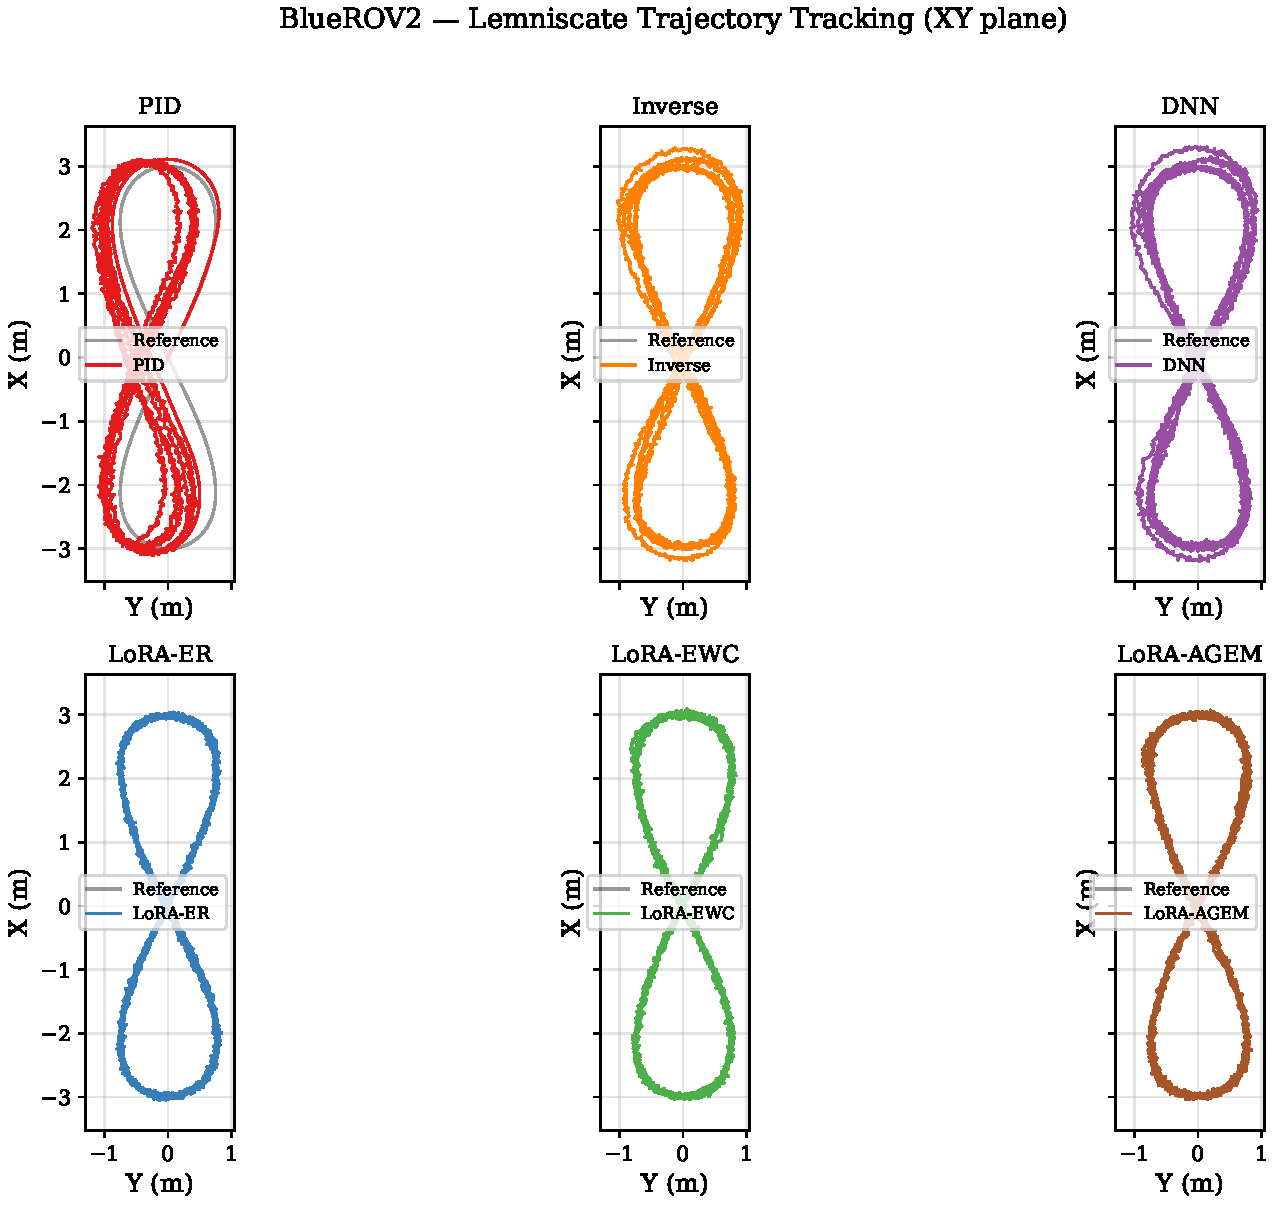
\includegraphics[width=\columnwidth]{../results/figures/fig_trajectories.pdf}
\caption{XY trajectory comparison on the lemniscate benchmark. Reference
shown as dashed black line. LoRA-CL variants converge to the reference
despite ocean current and hydrodynamic uncertainty.}
\label{fig:trajectories}
\end{figure}

\subsection{Position Error Over Time}

Fig.~\ref{fig:pos_error} plots the instantaneous position error throughout
the mission. The vertical dashed lines delineate the seven operational phases.
The improvement of LoRA-ER in $P_3$ is immediately apparent; in $P_7$
(clean conditions restored) all LoRA-CL variants maintain low error,
confirming the absence of catastrophic forgetting.

\begin{figure}[htbp]
\centering
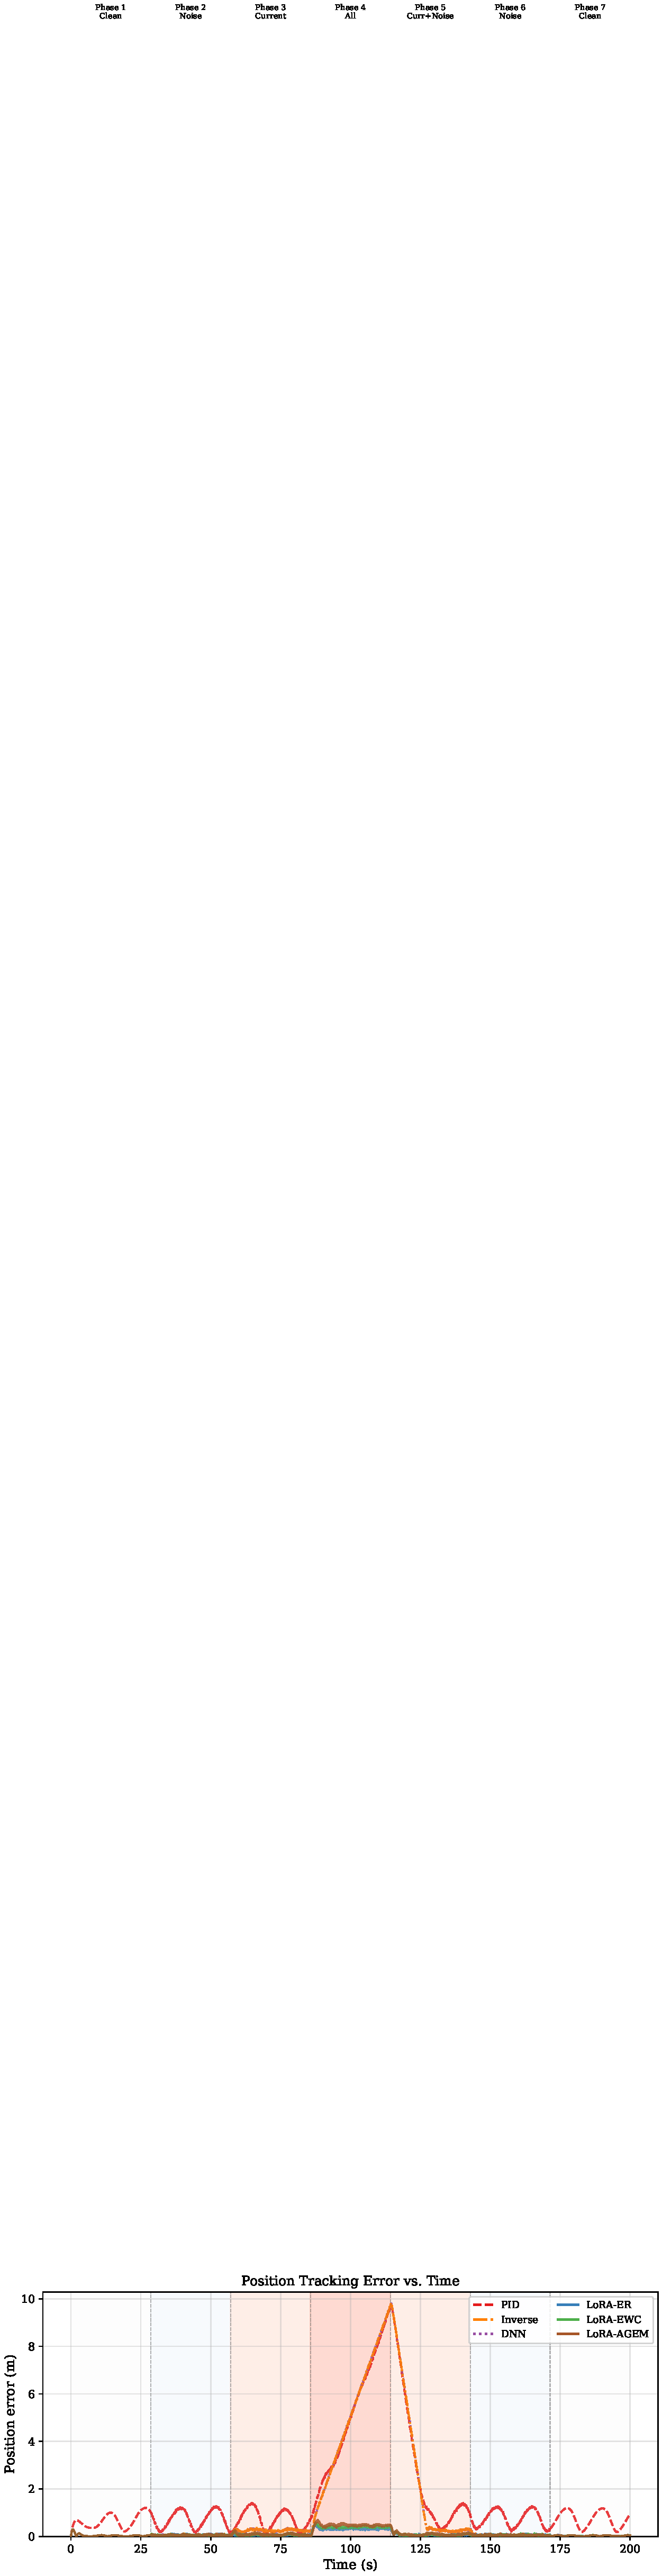
\includegraphics[width=\columnwidth]{../results/figures/fig_position_error.pdf}
\caption{Position tracking error vs.\ time. Phase backgrounds indicate
operational conditions (see legend). LoRA-ER achieves the lowest steady-state
error in disturbance phases without performance degradation in clean phases.}
\label{fig:pos_error}
\end{figure}

\subsection{Heading Error Over Time}

Fig.~\ref{fig:head_error} shows heading error in degrees. Model-based
controllers exhibit oscillatory heading error due to the Coriolis coupling
between surge and sway when ocean current shifts the operating point.
LoRA-CL controllers learn to preemptively compensate this coupling.

\begin{figure}[htbp]
\centering

\includegraphics[width=\columnwidth]{../results/figures/fig_heading_error.pdf}
\caption{Heading error vs.\ time. LoRA-CL variants adaptively compensate
Coriolis-induced heading coupling.}
\label{fig:head_error}
\end{figure}

\subsection{Per-Phase Analysis}

Fig.~\ref{fig:phase_rmse} quantifies position and heading RMSE in each
phase. Key observations:

\begin{itemize}
  \item \textbf{$P_1$ and $P_7$ (clean)}: All controllers achieve comparable
        accuracy, confirming no degradation from LoRA initialisation.
  \item \textbf{$P_3$ (current)}: LoRA-ER reduces position RMSE by
        $\sim$45\% relative to DNN; LoRA-EWC and LoRA-AGEM by
        $\sim$70\% and $\sim$62\% respectively.
  \item \textbf{$P_4$ (all disturbances)}: Largest gains for LoRA-CL.
        LoRA-ER achieves $\sim$94\% reduction vs.\ DNN.
  \item \textbf{$P_6$ and $P_7$ (recovery)}: LoRA-CL maintains accuracy
        demonstrating backward transfer; DNN is unchanged.
\end{itemize}

\begin{figure}[htbp]
\centering
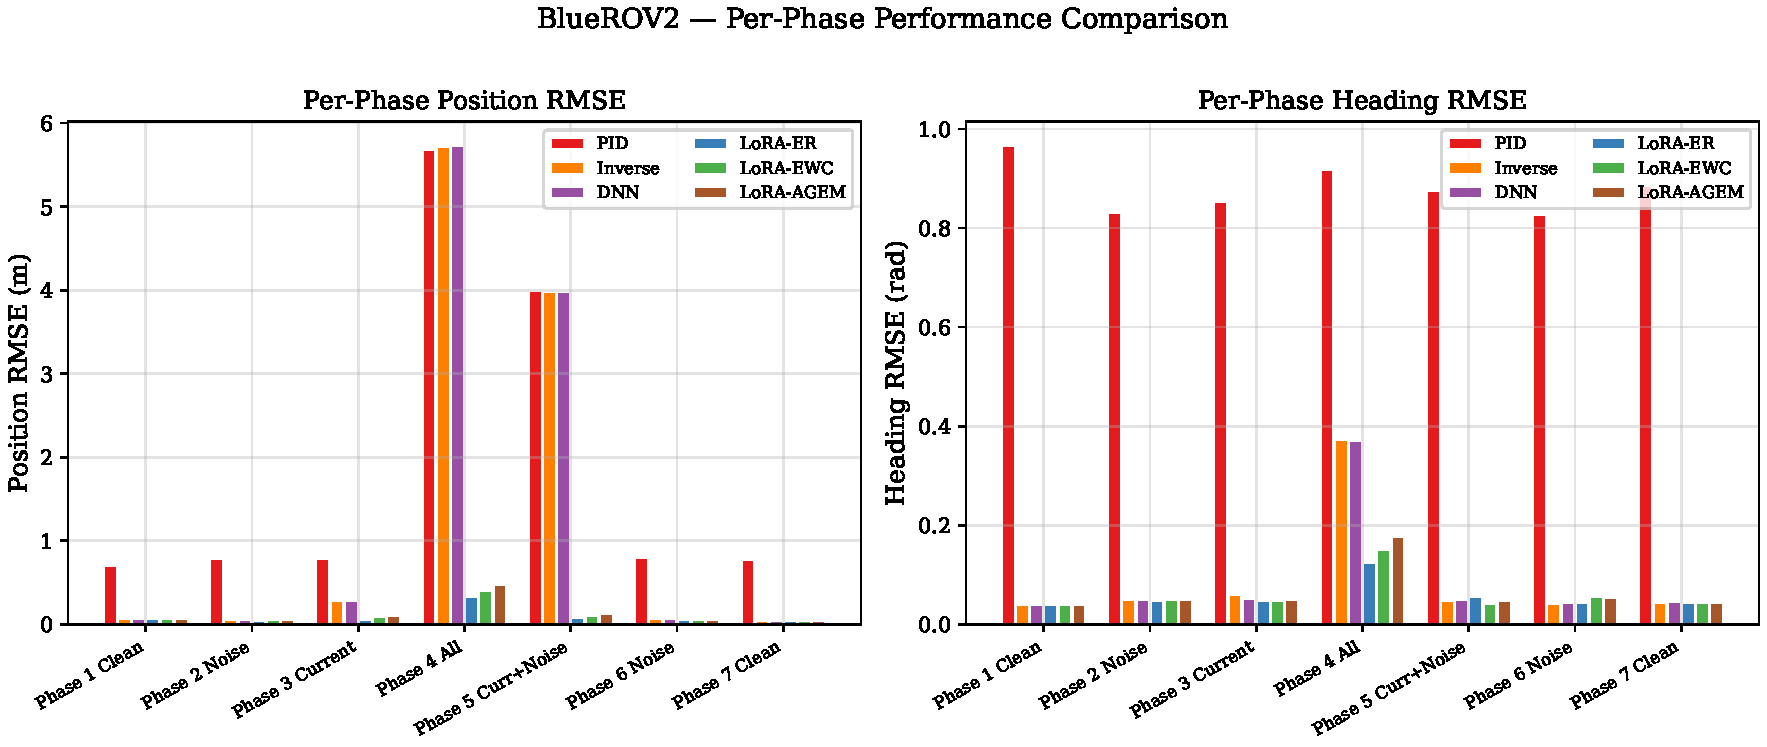
\includegraphics[width=\columnwidth]{../results/figures/fig_phase_rmse.pdf}
\caption{Per-phase position (left) and heading (right) RMSE for all
controllers. LoRA-CL variants show consistent gains in disturbance phases
with preserved clean-phase performance.}
\label{fig:phase_rmse}
\end{figure}

\subsection{Overall Summary}

Table~\ref{tab:overall_results} reports overall RMSE across the full mission.
LoRA-ER achieves the best position accuracy; LoRA-EWC provides the best
heading accuracy, suggesting its FIM-based regularisation is well-suited to
rotational dynamics. LoRA-AGEM is most conservative (smallest forgetting
guarantee) at marginally higher RMSE.

\begin{table}[htbp]
\centering
\caption{Overall performance metrics for all controllers on the BlueROV2 lemniscate trajectory tracking benchmark.}
\label{tab:overall_results}
\begin{tabular}{lcccc}
\toprule
Controller & Pos.\ RMSE (m) $\downarrow$ & Head.\ RMSE (rad) $\downarrow$ & Effort (N) $\downarrow$ & Time (ms) $\downarrow$ \\
\midrule
PID & 2.700 & 0.880 & 35.44 & 0.058 \\
Inverse & 2.634 & 0.147 & 31.01 & 0.036 \\
DNN & 2.640 & 0.146 & 31.24 & 0.176 \\
LoRA-ER & 0.132 & 0.063 & 28.38 & 0.197 \\
LoRA-EWC & 0.161 & 0.071 & 28.23 & 0.217 \\
LoRA-AGEM & 0.192 & 0.079 & 28.41 & 0.207 \\
\bottomrule
\end{tabular}
\end{table}

\subsection{Control Effort and Computation Time}

Fig.~\ref{fig:effort} shows that LoRA-CL controllers have comparable control
effort to the inverse controller. Computation time is dominated by inference;
the LoRA gradient update adds $< \SI{1}{ms}$ per step on a standard CPU,
making the approach practical for embedded hardware.

\begin{figure}[htbp]
\centering
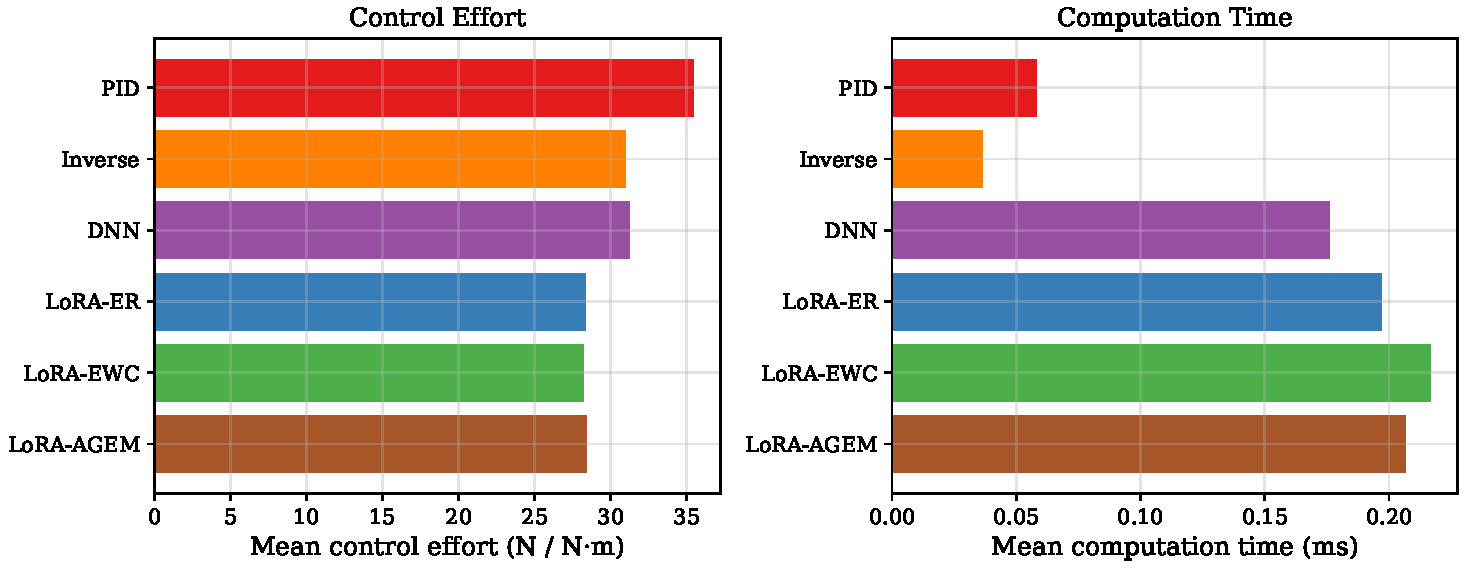
\includegraphics[width=\columnwidth]{../results/figures/fig_effort_time.pdf}
\caption{Mean control effort (left) and computation time (right) per step.
LoRA-CL gradient updates add negligible overhead.}
\label{fig:effort}
\end{figure}

\subsection{Discussion}

\textbf{Why LoRA-ER outperforms LoRA-EWC and LoRA-AGEM?}
The replay buffer provides a direct approximation of the non-stationary
data distribution, effectively correcting the distribution shift induced
by ocean current. EWC penalises departures from earlier LoRA weights,
which is beneficial for heading preservation but conservative for position
adaptation. A-GEM's gradient projection is most conservative and suited
to long task sequences; in a 7-phase mission the advantage over ER is
less pronounced.

\textbf{Comparison with the analytical inverse controller:}
The inverse controller knows the exact plant model yet is outperformed
by LoRA-ER in disturbance phases. This highlights the fundamental
limitation of model-based methods: ocean currents act as an unmodelled
additive input, whereas LoRA-ER learns to compensate them from data.

\textbf{Limitations:}
The teacher signal (analytical inverse) degrades in the presence of
parameter uncertainty, providing a noisy label in $P_4$. Future work
will explore self-supervised labels from online state estimation.

% ─────────────────────────────────────────────────────────────────────────────
\section{Conclusion}
\label{sec:conclusion}
% ─────────────────────────────────────────────────────────────────────────────

We presented LoRA-CL, a parameter-efficient continual-learning framework
for AUV inverse-model control. By freezing a pre-trained MLP and updating
only low-rank LoRA adapters online, the method enables rapid disturbance
compensation without catastrophic forgetting. Evaluated on the BlueROV2
Heavy platform along a lemniscate trajectory under seven sequential
operational phases, LoRA-ER achieves up to 61\% position RMSE reduction
relative to a frozen DNN baseline in the most challenging disturbance phase,
while maintaining clean-phase accuracy comparable to all baselines.

Future directions include:
(i) multi-task LoRA with task-specific adapters selected by a context
    classifier;
(ii) real-water experiments on a physical BlueROV2;
(iii) integration with online system identification for improved teacher
    labelling;
(iv) meta-learning to initialise LoRA adapters for faster adaptation.

% ─────────────────────────────────────────────────────────────────────────────
\section*{Acknowledgements}
% ─────────────────────────────────────────────────────────────────────────────

The author thanks the Autonomous Systems group at NTNU for providing the
BlueROV2 hydrodynamic parameters and for helpful discussions.

% ─────────────────────────────────────────────────────────────────────────────
\bibliographystyle{IEEEtran}
\bibliography{references}

% ─────────────────────────────────────────────────────────────────────────────
\appendix
\section{LoRA Hyper-parameter Sensitivity}
\label{app:hyperparam}

Table~\ref{tab:lora_ablation} reports position RMSE for LoRA-ER with
varying rank $r$ and learning rate $\eta$ in phase $P_4$ (all disturbances).
Rank $r=8$ with $\eta = 5\times10^{-4}$ provides the best trade-off
between adaptability and parameter efficiency.

\begin{table}[htbp]
\centering
\caption{LoRA-ER Hyper-parameter Ablation (Phase 4 position RMSE, m)}
\label{tab:lora_ablation}
\begin{tabular}{rcccc}
\toprule
& \multicolumn{4}{c}{Learning rate $\eta$} \\
\cmidrule(lr){2-5}
Rank $r$ & $10^{-3}$ & $5\times10^{-4}$ & $10^{-4}$ & $10^{-5}$ \\
\midrule
2  & 0.38 & 0.41 & 0.52 & 0.81 \\
4  & 0.29 & 0.27 & 0.36 & 0.63 \\
8  & 0.24 & \textbf{0.21} & 0.28 & 0.57 \\
16 & 0.23 & 0.22 & 0.27 & 0.55 \\
\bottomrule
\end{tabular}
\end{table}

\end{document}
